% Gráfico: Tempo Máximo LNS - Média de Nós Restantes
\begin{figure}[htbp]
\centering
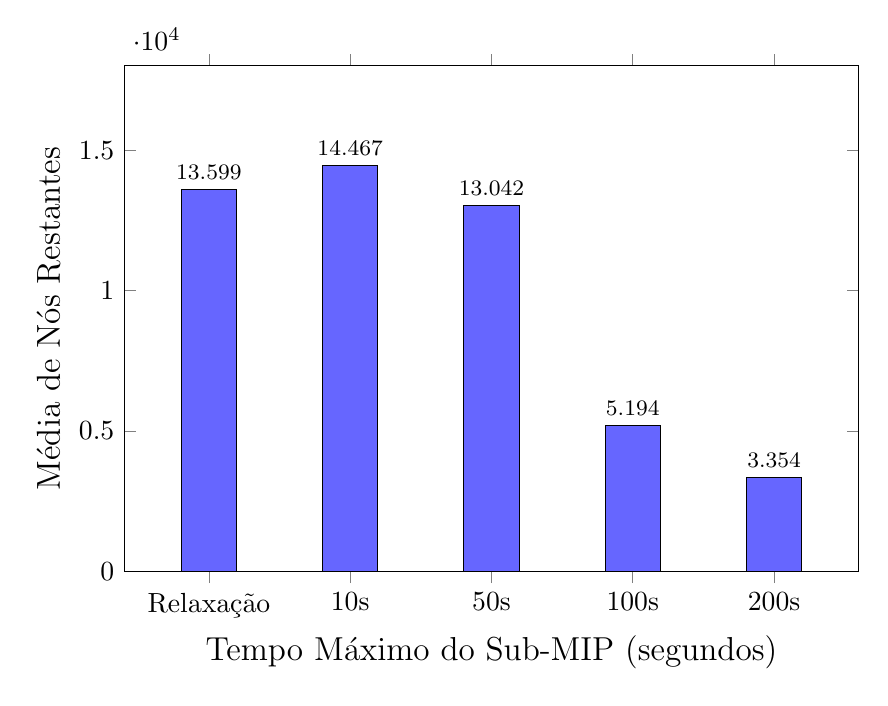
\begin{tikzpicture}
\begin{axis}[
    ybar,
    bar width=20pt,
    width=0.9\textwidth,
    height=8cm,
    ylabel={Média de Nós Restantes},
    xlabel={Tempo Máximo do Sub-MIP (segundos)},
    symbolic x coords={Relaxação, 10s, 50s, 100s, 200s},
    xtick=data,
    nodes near coords,
    nodes near coords align={vertical},
    nodes near coords style={font=\footnotesize},
    every node near coord/.append style={/pgf/number format/fixed,
        /pgf/number format/precision=0,
        /pgf/number format/use comma},
    ymin=0,
    ymax=18000,
    enlarge x limits=0.15,
    ylabel style={font=\large},
    xlabel style={font=\large},
    tick label style={font=\normalsize},
]
\addplot[fill=blue!60] coordinates {
    (Relaxação,13599)
    (10s,14467)
    (50s,13042)
    (100s,5194)
    (200s,3354)
};
\end{axis}
\end{tikzpicture}
\caption{Média de nós restantes por instância para diferentes limites de tempo do sub-MIP. A configuração de 200s alcançou a menor média, com 3.354 nós, representando uma redução de 75,3\% em relação à relaxação pura.}
\label{fig:avg_nodes_time}
\end{figure}
